\documentclass[11pt]{article}
\usepackage[margin=1in]{geometry}
\usepackage{graphicx,booktabs,amsmath,amssymb,xcolor,caption,subcaption}
\usepackage[hidelinks]{hyperref}
\usepackage{times}
\captionsetup{font=small,labelfont=bf}

\title{\textbf{Two Tiny Brains in a Fluid:\\ Laptop-Scale Reinforcement Learning for
Navigation and Gait Discovery\\ in Exactly-Solved Flows}}
\author{Rajat Dandekar\\ \small Vizuara AI Labs\\
\small RL in Production --- Bonus Lecture}
\date{\today}

\begin{document}
\maketitle

\begin{abstract}
\noindent
We present two fully replicable, laptop-scale demonstrations of reinforcement learning
applied to fluid mechanics, intended as a bonus lecture for a bootcamp whose main track
trains language models with GRPO. Both use tabular Q-learning, pure \texttt{numpy}, and
flows with exact or semi-analytic physics, so that all compute goes into learning and
every claim is checkable in minutes. \textbf{Problem 1 (navigation):} a robot swimming at
$v_s = 0.3$ must cross a Taylor--Green vortex lattice whose currents reach $U = 1.0$.
The honest baseline --- aim straight at the target, drawn from the agent's own eight-action
compass --- arrives only $57.9\%$ of the time; the remainder are swept into closed orbits.
A $144\times 8$ Q-table reaches $\mathbf{100\%}$ arrival, discovering tacking detours and
routes that exploit the domain's periodicity. \textbf{Problem 2 (gait):} the
Najafi--Golestanian three-sphere swimmer, integrated with force-free Oseen hydrodynamics
at every substep, must learn how to move at all against Purcell's scallop theorem. An
\emph{eight-number} Q-table invents, from reward alone, a four-beat crawl --- squeeze one
arm, squeeze the other, stretch the first, stretch the second, like an inchworm --- which is
precisely the non-reciprocal cycle Najafi \& Golestanian derived by hand in 2004. The
reciprocal baseline (flapping one arm back and forth) measures $-0.0003$ body displacements
over 24 strokes --- the theorem confirmed by
our own physics --- against $+0.103$ for the learned gait. We also report the instructive
failure that preceded these results: a gyrotactic torque-control task in which an
exact-MDP oracle proved that no policy expressible in any observation we tried could beat
the naive swimmer by more than $25\%$ --- the bottleneck was control authority, not the
learning algorithm. We argue this oracle-first debugging pattern is the transferable
lesson of the whole exercise.
\end{abstract}

\section{Motivation}

The main lectures of this bootcamp train billion-parameter language models with
reinforcement learning. The loop --- observe, act, receive a verifiable reward, update ---
is entirely general, and nothing teaches that generality like pointing the same loop at
a different century of physics. Fluid mechanics is an ideal target: the physics is
unforgiving (there is no reward-hacking a conservation law), rewards are verifiable by
construction, and there exist flows whose solutions are exact, so the ``simulator'' is
two lines of \texttt{numpy} and training takes minutes on a laptop.

Both problems below replicate published work at reduced scale: Zermelo navigation by RL
(Biferale et al., 2019) and RL gait discovery for the three-sphere swimmer (Tsang et al.,
2020; the swimmer itself from Najafi \& Golestanian, 2004).

\section{Problem 1: Zermelo navigation}

\subsection{Setup}

The flow is the Taylor--Green lattice, an exact steady solution of the incompressible
equations on the periodic square $[0, 2\pi)^2$:
\begin{equation}
u_x = U\cos x \sin y, \qquad u_y = -U\sin x \cos y, \qquad U = 1.
\end{equation}
A robot at position $\mathbf{x}$ moves with $\dot{\mathbf{x}} = \mathbf{u}(\mathbf{x}) +
v_s\,\hat{\mathbf{e}}_a$, where $\hat{\mathbf{e}}_a$ is one of eight compass headings and
$v_s = 0.3$: the current is more than three times faster than the swimmer. Starting near
$(1.2, 1.2)$ (with jitter), it must reach a disc of radius $0.45$ at $(5.2, 5.2)$.

\textbf{MDP.} State: the robot's cell in a $12\times12$ partition of the domain ---
position only; the agent cannot sense the flow. Action: one of 8 headings, held for
$0.2$ time units. Reward: $-1$ per decision, $+200$ on arrival; episodes cap at 400
decisions. This is Sutton \& Barto's \emph{windy gridworld} with the wind replaced by a
real incompressible flow that can locally overpower the agent.

\textbf{Baseline.} The naive policy aims straight at the target (periodic-aware), choosing
the nearest of the same 8 headings --- a genuine member of the agent's action space.

\subsection{Training and results}

Episodic Q-learning ($\gamma = 0.995$, lr $0.2$, $\varepsilon$: $0.4 \to 0.01$), with 512
robots exploring in parallel and averaging their TD updates into one shared table; 300
generations train in about 90 seconds.

\begin{table}[h]
\centering
\begin{tabular}{lcc}
\toprule
 & arrival rate & median time (arrivers only) \\
\midrule
naive (aim at target) & 57.9\% & 18 decisions \\
\textbf{Q-learned} & \textbf{100.0\%} & 21 decisions \\
\bottomrule
\end{tabular}
\caption{Evaluation on 4{,}000 fresh-seed episodes each. The naive median is
survivor-biased: it averages only the lucky 58\%.}
\end{table}

The qualitative finding matters more than the numbers: the learned policy \emph{tacks}.
Robots first swim away from the target, ride a favourable jet across the lattice, and
enter from the far side; some routes wrap the periodic boundary because that direction
travels with the current. Figure~\ref{fig:traj} shows both behaviours; the full policy is
small enough to plot in its entirety as one arrow per map cell.

\begin{figure}[h]
\centering
\begin{subfigure}{0.32\textwidth}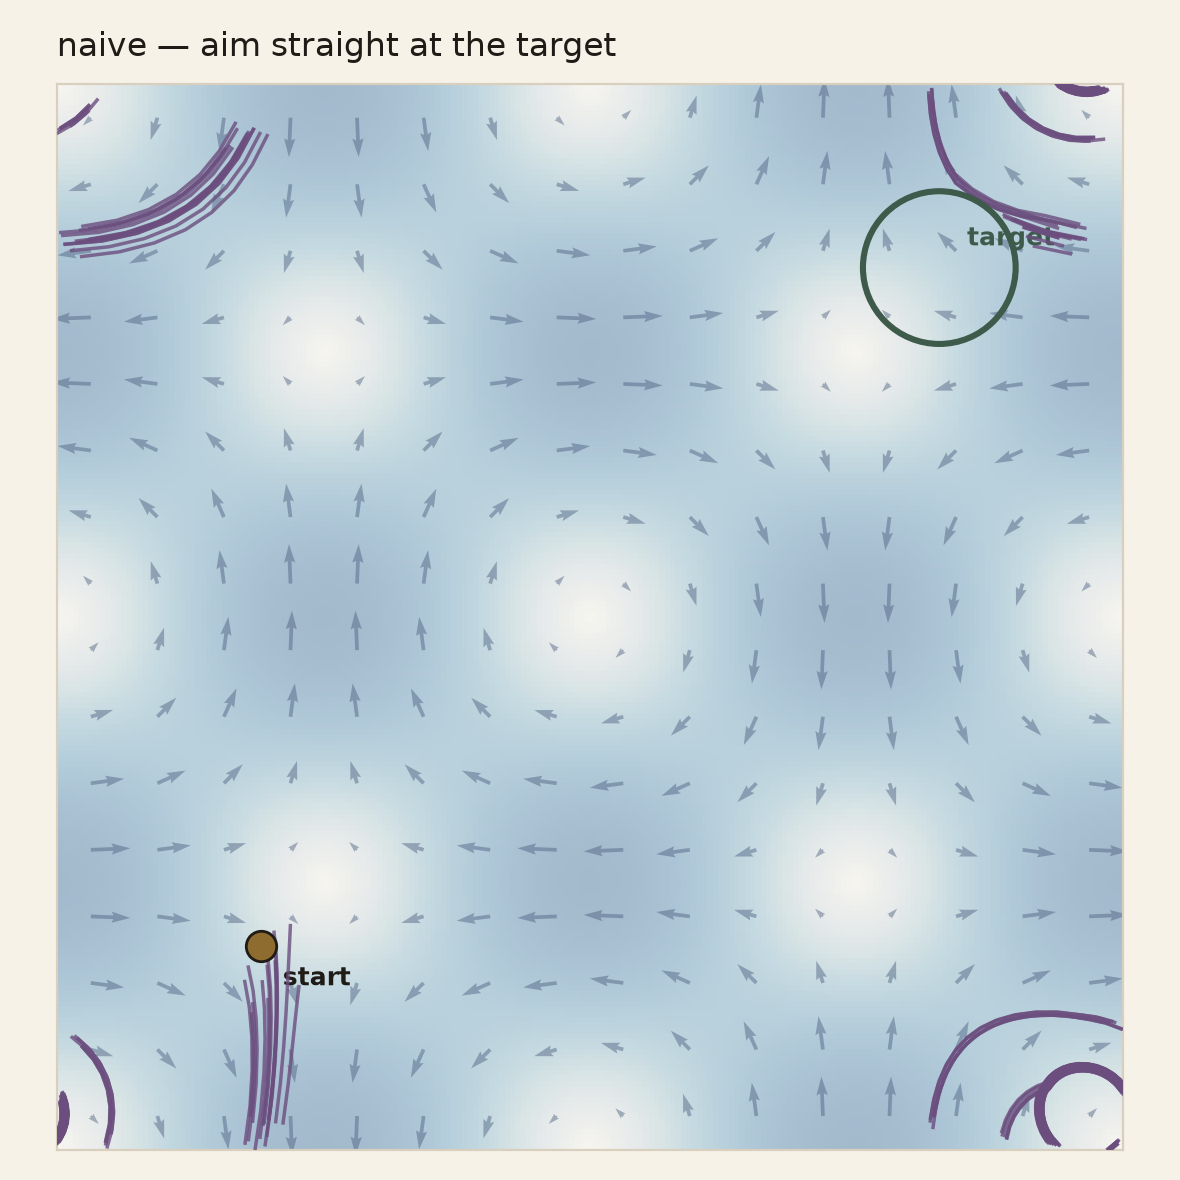
\includegraphics[width=\textwidth]{../figures/nav_traj_naive.png}\end{subfigure}
\begin{subfigure}{0.32\textwidth}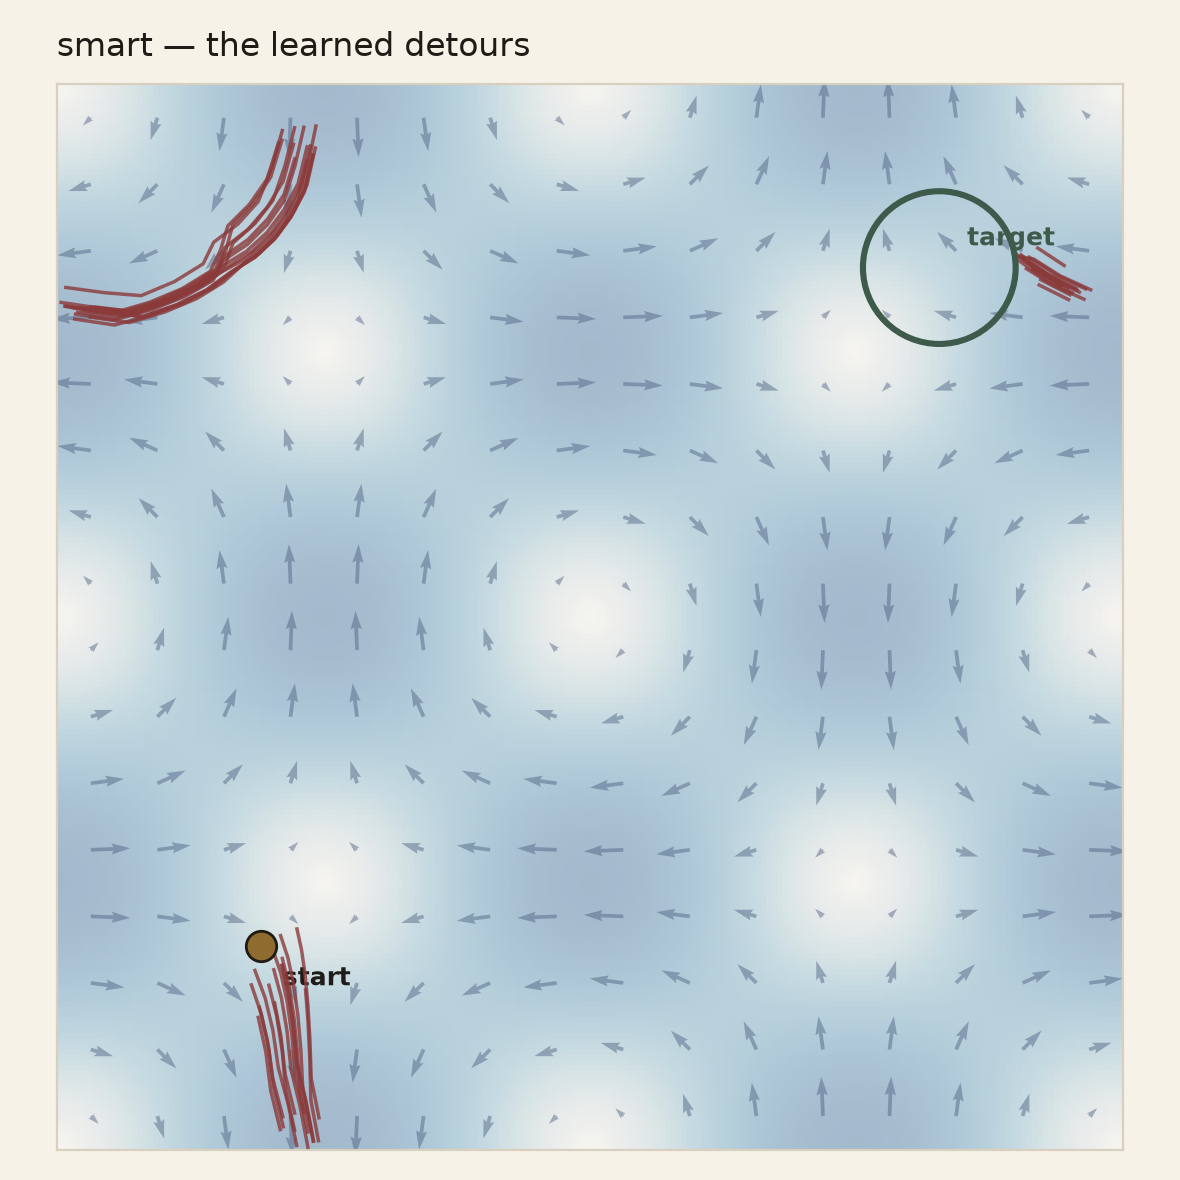
\includegraphics[width=\textwidth]{../figures/nav_traj_smart.png}\end{subfigure}
\begin{subfigure}{0.32\textwidth}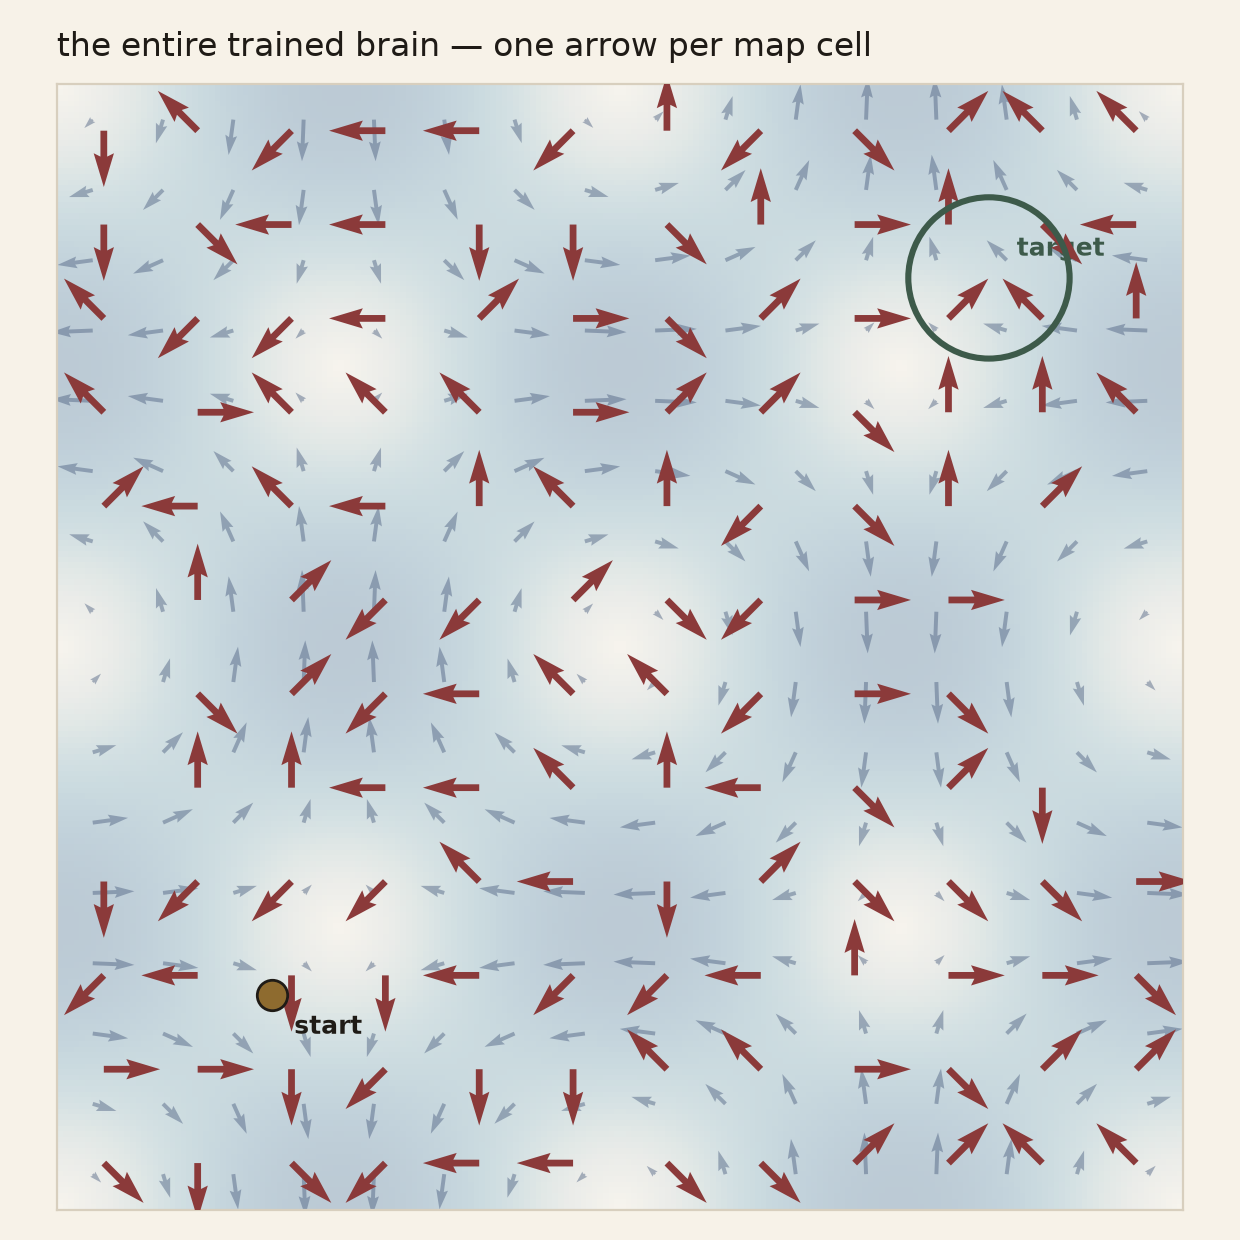
\includegraphics[width=\textwidth]{../figures/nav_policy_field.png}\end{subfigure}
\caption{Left: naive trajectories --- deflected, swept past the goal, trapped in closed
orbits (tight spirals). Centre: learned detours. Right: the entire trained policy, one
arrow per cell.}
\label{fig:traj}
\end{figure}

RL's win here is \emph{reliability}, not speed --- the same quantity it bought in the
bootcamp's language-model experiments. Where the opposing jet exceeds $v_s$, no amount of
effort helps; only a route does.

\section{Problem 2: learning a gait against the scallop theorem}

\subsection{Physics}

At low Reynolds number the Stokes equations are time-reversible: any reciprocal
(retraced) stroke yields exactly zero net displacement (Purcell, 1977). The simplest
swimmer that evades the theorem is Najafi \& Golestanian's: three spheres of radius
$a = 0.1$ on a line, joined by two arms of length $L = 1$ (extended) or $L - \epsilon$
with $\epsilon = 0.4$ (contracted).

We integrate the honest hydrodynamics. With sphere forces $f_i$ along the line, Oseen
mobility gives $v_i = f_i/(6\pi\mu a) + \sum_{j\neq i} f_j / (4\pi\mu r_{ij})$; arm
motions prescribe $v_2 - v_1$ and $v_3 - v_2$, and the swimmer is force-free
($\sum f_i = 0$). This is three linear equations solved at every Euler substep;
displacement per stroke \emph{emerges} and is never looked up.

\subsection{MDP and results}

State: the arm configuration, $(\text{arm}_1, \text{arm}_2) \in \{C, E\}^2$ --- four
states. Action: toggle one arm --- two actions. Reward: signed centre-of-mass
displacement during the stroke. The complete policy is a $4\times2$ table:
\textbf{eight numbers}.

Q-learning ($\gamma = 0.9$, 300 episodes of 24 strokes, $\sim$40 s) converges to a
four-beat crawl: squeeze the left arm, squeeze the right, stretch the left, stretch the
right, repeat --- the shape of the machine travels a \emph{loop} that never retraces
itself, the way an inchworm bunches and extends. In the standard notation this is the cycle
$(E,E) \to (C,E) \to (C,C) \to (E,C) \to \cdots$, precisely the stroke Najafi \&
Golestanian derived analytically; here it is discovered from reward alone. Over 24
strokes:

\begin{center}
\begin{tabular}{lc}
\toprule
gait & net displacement \\
\midrule
reciprocal (toggle one arm forever) & $-0.0003$ \\
\textbf{learned cycle} & $\mathbf{+0.103}$ \\
\bottomrule
\end{tabular}
\end{center}

The reciprocal number is the scallop theorem confirmed by our own integrator (it is
round-off-scale, $\sim$350$\times$ smaller than the learned gait). The learned
displacement per cycle ($\approx 0.017$) agrees with the Najafi--Golestanian asymptotic
$\Delta \sim a\,\epsilon^2/L^2 \approx 0.016$ to the $O(1)$ factor expected at our
non-infinitesimal $\epsilon/L = 0.4$.

\section{The instructive failure}

Our first formulation was harder and more biological: a \emph{gyrotactic} swimmer
(bottom-heavy, righting toward ``up'' with timescale $B$) whose RL action biases the
righting direction --- after Colabrese et al.\ (2017). In the regime where the naive
swimmer visibly struggles ($B = 8$), vortex spin exceeds the control torque by a factor
of $\sim$16, and Q-learning plateaued at zero improvement.

Rather than tune hyperparameters indefinitely, we used an \textbf{exact-MDP oracle}:
collect transitions under uniform-random actions, fit the empirical transition matrix
over the discrete states, and solve it by relative value iteration. Whatever policy this
produces is the best the observation can express, independent of any learning dynamics.
The oracle's verdict, across every observation we tried (local vorticity + heading, 12
states; adding an updraft bit, 24; flow-sign features, 16): the \emph{optimal} policy
gains only $9$--$25\%$ over naive. Sensing richer features did not help; switching the
\emph{actuation} to direct heading control changed the problem completely and made
Problem 1 what it is.

Three lessons, in decreasing order of importance: \textbf{control authority} decides
whether learning is possible; \textbf{observation design} decides how much of the
achievable gain is expressible; the \textbf{algorithm} only decides how fast you approach
that ceiling. And the debugging pattern generalises: for any tabular problem, solve the
MDP exactly before blaming the learner.

\section{Reproducibility}

Everything runs from two commands on a laptop (\texttt{numpy} + \texttt{matplotlib}
only); training takes $\sim$90\,s (navigation) and $\sim$40\,s (gait). All figures,
including the animations, regenerate from \texttt{scripts/make\_result\_figures.py}.
Code, trained tables, and per-run summaries accompany this report.

\begin{thebibliography}{9}
\bibitem{biferale} L. Biferale, F. Bonaccorso, M. Buzzicotti, P. Clark Di Leoni,
K. Gustavsson. \emph{Zermelo's problem: optimal point-to-point navigation in 2D
turbulent flows using reinforcement learning}. Chaos 29, 103138 (2019).
\bibitem{colabrese} S. Colabrese, K. Gustavsson, A. Celani, B. Mehlig. \emph{Flow
navigation by smart microswimmers via reinforcement learning}. PRL 118, 158004 (2017).
\bibitem{ng} A. Najafi, R. Golestanian. \emph{Simple swimmer at low Reynolds number:
three linked spheres}. PRE 69, 062901 (2004).
\bibitem{tsang} A. C. H. Tsang, P. W. Tong, S. Nallan, O. S. Pak. \emph{Self-learning
how to swim at low Reynolds number}. Phys. Rev. Fluids 5, 074101 (2020).
\bibitem{purcell} E. M. Purcell. \emph{Life at low Reynolds number}. Am. J. Phys. 45, 3
(1977).
\bibitem{reddy} G. Reddy, A. Celani, T. J. Sejnowski, M. Vergassola. \emph{Learning to
soar in turbulent thermal environments}. PNAS 113, E4877 (2016).
\end{thebibliography}

\end{document}
